\chapter{其他}
\begin{introduction}[本章内容提要]
	\item 勾股数组
	\item 圆上整点与高斯素数
	\item 模线性方程循环节
	\item 分数转小数
	\item DFS Similar
	\item FFT, NTT
	%\item 多项式相关
\end{introduction}

\section{勾股数组}

\begin{definition}{本原勾股数组}{label}
	本原勾股数组是一个三元组$(a,b,c)$,其中$a,b,c$没有公因数,且满足:
	$$a^2 + b^2 = c^2$$
\end{definition}

\begin{theorem}{勾股数组定理}{gougushuzu}
	每个本原勾股数组$(a,b,c)\ $(a为奇数,b为偶数)都可从如下公式得出:
	$$
	a=st ,\quad  b=\frac{s^2-t^2}{2},\quad  c=\frac{s^2+t^2}{2}
	$$
	其中$s>t>=1$是任意没有公因数的奇数。
\end{theorem}


\section{平方数之和、圆上整点}
这一节要解决的问题是给定一个数$x$,判断它能否分解为两个整数的平方之和,以及具体来说如何分解。从几何意义上考虑就是以原点为圆心,$\sqrt{x}$为半径的圆,是否经过坐标点(横纵坐标都是整数),
以及具体是哪些点。

先从$x$为素数考虑,这个时候规律相对简单。
\subsection{将素数分解为平方之和}



\begin{theorem}{定理}{primesquare}
	设$p$是素数,则$p$是两平方数之和的充要条件是$p\equiv 1 \ (mod \ 4)   $ 或$p=2$。
\end{theorem}

\begin{proof}
这里有两个断言:
\begin{itemize}
	\item $p$是两平方数之和;
	\item $p\equiv 1\ (mod\ 4)$ 或者 $p=2$。
\end{itemize}

要证明充要性有两个方面,即用一个断言作为条件去证明另外一个,下面分别证明。
\begin{enumerate}
	\item 若$p$是两平方数之和,则$-a^2\equiv b^2 (mod \ p)$ ,接着对两边取勒让德符号:(回顾第四章的内容)
	\begin{align*}
	\left(\frac{-1}{p}\right)\left(\frac{a}{p}\right)^2&=\left(\frac{b}{p}\right)^2 \\
	\left(\frac{-1}{p}\right)&=1
	\end{align*}
	于是由二次互反律知,$p$模4余1或者$p=2$。$\square$
	\item 当$p\equiv 1\ (mod\ 4)$或$p=2$时,要证明$p$一定可以表示成两平方数之和。也就是说只要我们能想到一种方法总能找到如何分解,就完成了证明。下面介绍一种方法,
	称之为{\heiti 费马降阶法(Fermat Descent Procedure)}。我们后面的代码就是基于此方法。
	
	我们从$A^2+B^2=Mp$开始,如果这里$M=1$,则证明完毕。所以我们考虑$M\ge 2$。
	费马的想法是,我们用现有的$A,B,M$,要是能构造出$a^2+b^2=mp \ \&\&\ m\le M-1$,
	则迭代下去,$m=1$时就完成了构造。

	在说具体的构造方法之前,先看一个恒等式,其正确性是显然的,在下面的构造过程中,这个恒等式起到关键作用。
	$$
	(u^2+v^2)(A^2+B^2)=(uA+vB)^2+(vA-uB)^2
	$$
	费马降阶法的过程如表\ref{tab:fermat-descent}所示:
	\begin{table}[!htbp]
		\centering
		\caption{费马降阶法 \label{tab:fermat-descent}}
		\begin{spacing}{1.5}
			\begin{tabular}{|c|c|}
				\toprule[1pt]
				举例(p=881) & 符号表示\quad p any prime $\equiv$ 1($mod\ 4$) \\
				\midrule[2pt]
				有$387^2+1^2=170*881$,$\ 170<881$ & 有$A^2+B^2=Mp$,$\ M<p$\\
				\midrule[1pt]
				\tabincell{c}{求得数$47,\ 1$使得\\$47\equiv 387\ (mod\ 170)$\\ $1\equiv 1\ (mod\ 170)$ \\ 其中$-\frac{170}{2}\le 47,1\le \frac{170}{2}$}  & 
				\tabincell{c}{求得数$u,\ v$使得\\$u\equiv A\ (mod\ M)$\\ $v\equiv B\ (mod\ M)$ \\ 其中$-\frac{M}{2}\le u,v\le \frac{M}{2}$}  \\
				\midrule[1pt]
				\tabincell{c}{于是有\\$47^2+1^2\equiv 387^2+1^2\equiv 0\ (mod\ 170)$}  & 
				\tabincell{c}{于是有\\$u^2+v^2\equiv A^2+B^2\equiv 0\ (mod\ M)$}  \\
				\midrule[1pt]
				\tabincell{c}{所以可写\\$47^2+1^2 = 170*13$ \\ $387^2+1^2 = 170*881$} & 
				\tabincell{c}{所以可写\\$u^2+v^2 = Mr(1\le r< M)$ \\ $A^2+B^2 = Mp$}  \\
				\midrule[1pt]
				\tabincell{c}{相乘可得\\$(47^2+1^2)(387^2+1^2) = 170^2*13*881$} & 
				\tabincell{c}{相乘可得\\$(u^2+v^2)(A^2+B^2) = M^2*r*p$}  \\
				\midrule[1pt]
				\multicolumn{2}{|c|}{利用恒等式$	(u^2+v^2)(A^2+B^2)=(uA+vB)^2+(vA-uB)^2 $} \\
				\midrule[1pt]
				\tabincell{c}{$(47*387+1*1)^2 + (1*387 - 47*1)^2$ \\ $=170^2*13*881$ \\ 所以$18190^2 + 340^2 = 170^2*13*881$} & 
				\tabincell{c}{$(uA+vB)^2+(vA-uB)^2 = M^2*r*p$}  \\
				\midrule[1pt]
				\tabincell{c}{两边同除以$170^2$得 \\ $(\frac{18190}{170})^2 + (\frac{340}{170})^2 = 13*881$ \\ $107^2 + 2^2 = 13*881$} & 
				\tabincell{c}{两边同除以$M^2$得 \\ $(\frac{uA+vB}{M})^2 + (\frac{vA-uB}{M})^2 = rp$ \\ (肯定可以整除) }  \\
				\midrule[1pt]
				\multicolumn{2}{|c|}{由此得到能表示成两平方数之和的$p$的更小倍数} \\
				\midrule[1pt]
				\multicolumn{2}{|c|}{重复上述过程,直到$p$本身能表成两平方数之和$(r=1)$} \\
				\bottomrule[1pt]
			\end{tabular}%
		\end{spacing}
	\end{table}%
	
	可以发现,每迭代一次,$p$的系数至少减半,即迭代次数为$O(logp)$次。为了说明上述过程的正确性,我们还要证明5个断言的正确性。
	\begin{enumerate}
		\item 一定可以找出数$A,B$,使得$A^2+B^2=Mp$,且$M<p$ 。
		\begin{proof}
			取同余式$x^2\equiv -1\ (mod \ p)$的一个解,由二次互反律知,当$p\%4=1$时,必定有解$x$。所以取
			$A=x,B=1$具有性质$p\ | \ A^2+B^2$,而且$M=\frac{A^2+B^2}{p}\le \frac{(p-1)^2+1^2}{p}<p$。
			$\square$ 
		\end{proof}
	\end{enumerate}


	在降阶程序的第二步,我们选取$u,v$使其满足
	$$
	u\equiv A (mod \ M),\quad v\equiv B(mod \ M), \quad -\frac{1}{2}M\le u,v\le \frac{1}{2}M
	$$
	于是有
	$$
	u^2+v^2\equiv A^2+B^2\equiv 0 \quad (mod \ M )
	$$
	设$u^2+v^2=rM$,其余四个断言如下:
	\begin{enumerate}[resume] % tell the enumerate to resume numbering
		\item $r\ge1$
		\item $r<M$ 
		\item $uA+vB$能被$M$整除
		\item $vA-uB$能被$M$整除
	\end{enumerate}
	这四个断言比较容易证明,这里不再给出。$\square$
\end{enumerate}
	至此,对定理\ref{thm:primesquare}的证明结束。$\square$
\end{proof}

\vbox{}

上面求解过程中关键的一步是求解$x^2\equiv -1 \ (mod \ p)$,可以直接使用二次剩余的模板,也可以使用随机算法。
即随机一个$a∈[1,p-1]$ ,求解$b\equiv a^{(p-1)/4}\ (mod\ p)$,由欧拉准则可知$b^2\equiv (\frac{a}{p}) \ (mod\ p)$,
即若选取的$a$不是$p$的二次剩余(有一半的概率),则求得的$b$即为解$x$。由二次剩余性质知有两个解$x_1,x_2$,且$x_1+x_2=p$。

代码如下:
\lstinputlisting[language=C++, style=codestyle2]{code07/random-algo-modsqr.cpp}

现在我们可以将素数分解为平方数之和了,下面看一下对于一般数该怎么做。

\subsection{将数分解为平方之和}
这一节的内容,不打算给出相关证明,而是给出一些结论和代码。因为我觉得下面这个视频已经讲的不错了,\href{https://www.bilibili.com/video/av12131743}{bilibili: 隐藏在素数规律中的$\pi$}。

\begin{theorem}{圆上整点数定理}{label}
	定义函数$\chi(n)$如下:
	\begin{align*}
		\chi(n) = \left\{\begin{matrix}
		1&  \quad  n\%4==1\\
		-1  & \quad  n\%4==3 \\
		0 &\quad   n\%4==0\ or\ 2
		\end{matrix}\right. \quad\quad n>0
	\end{align*}
	对于半径为$\sqrt{N}$的圆,圆上整点的数目(即将$N$分成两个平方数之和的方案数)可以这样计算:
	
	将$N$质因数分解:
	$$
	N = p_1^{k_1}*p_2^{k_2}*...*p_m^{k_m}
	$$
	则圆上整点数目 = $4*\Pi_{i=1}^{m}(\sum_{j=0}^{k_i}\chi(p_i^j))$。
	
	上面的这个式子只是为了统一,所以看起来规律不明显。实际上一句话:
	
	如果有模4余3的素数的指数为奇数,则答案为0;否则就是所有模4余1的素数的指数加1后乘起来最后再乘4。
\end{theorem}

\vbox{}

至于具体如何计算分解的方案,推荐大家看上面那个视频。大致思路就是对于可分解的素数利用费马降阶法进行分解,然后再在复数域中对不同质数
的结果组合计算一下。下面给出代码:

输入一个半径$r$,输出在圆上的所有整点。

{\heiti 时间复杂度:$O(A+B)$,其中$A$为质因子分解$r^2(thus\ r)$的时间,$B$为圆上整点数。

该代码在$r\le 10^9$时通过测试,更大时注意下会不会爆范围。}

\href{https://nanti.jisuanke.com/t/41421}{圆上整点/高斯素数 \quad 2019上海网络赛 Peekaboo}

\lstinputlisting[language=C++, style=codestyle2]{code07/Lattice-points.cpp}






\section{循环节问题}
\subsection{二阶常系数齐次线性递推循环节}
所谓二阶常系数齐次线性递推式就是类似斐波那契递推式那样的数列。这样的数列在模意义下会存在循环节。下面阐述下如何求其循环节:


先将模数分解,在模素数幂意义下分别求循环节,最后取最小公倍数即可。而对于模素数幂有结论$G(p_i^{a_i}) = p_i^{a_1-1}G(p_i)$。$G(m)$表示在模数为$m$时的循环节大小。

所以问题转为模素数如何处理。即给定$a,b,f(1),f(2)$,且满足$f(n)=a*f(n-1) + b*f(n-2)$。求$f(n)\ mod\ p$的循环节。

写成矩阵形式,如下:
$$
\left[\begin{array}{c}{f(n)} \\ {f(n-1)}\end{array}\right]=\left[\begin{array}{cc}{a} & {b} \\ {1} & {0}\end{array}\right]\left[\begin{array}{c}{f(n-1)} \\ {f(n-2)}\end{array}\right]
$$

变形一下:
$$
\left[\begin{array}{c}{f(n+2)} \\ {f(n+1)}\end{array}\right]=\left[\begin{array}{cc}{a} & {b} \\ {1} & {0}\end{array}\right]^{n}\left[\begin{array}{c}{f(2)} \\ {f(1)}\end{array}\right]
$$
那么现在的问题就转化为求最小的$n$,使得
$$
\left[\begin{array}{ll}{a} & {b} \\ {1} & {0}\end{array}\right]^{n}(\bmod p)=\left[\begin{array}{ll}{1} & {0} \\ {0} & {1}\end{array}\right]
$$

如何快一点求$n$呢?这里直接给出结论:设$c=a^2+4b$, 有两种情况:
\begin{enumerate}
	\item 若$c$是模$p$的二次剩余,则$n$是$p-1$的因子;
	\item 若$c$不是模$p$的二次剩余,则$n$是$(p+1)(p-1)$的因子
\end{enumerate}
所以只要枚举因子并判断即可。
时间复杂度$O(T*2^3*log(p))$,其中$T$为$p-1$或$(p+1)(p-1)$的因子数目。

\subsection{分数小数的循环节}
\begin{custom}{问题}
给定一个分数$\frac{p}{q}$,将其转化为小数。
\end{custom}

\begin{solution}
考虑一个分数,有以下三种情况:
\begin{itemize}
	\item 整数
	\item 有限小数
	\item 无限循环小数
\end{itemize}

先来考虑下无限循环小数,我们先将$p$和$q$公共的因子除去,然后利用循环这个性质,可知存在$i,j$满足,$p*10^i \equiv p*10^j \ (mod \ q), \ where\ j>i\ge0$。
{\heiti 这里$i$代表循环出现前有多少位数,$j-i$表示循环节长度。}
化简后得$p*10^i*(10^{j-i}-1) \equiv 0\   (mod \ q)$。也就是说,$q\ |\ p*10^i*(10^{j-i}-1)$。由于$10^{j-i}-1$中一定不存在因子$2$和$5$,所以要想是$q$的倍数,
$2$和$5$的贡献均来自$10^i$。于是我们记录$q$中$2$的次幂数为$num2$,$5$的次幂数为$num5$,则$i = max(num2,num5)$。记$q$除去所有$2$和$5$因子后,为$m$,则$10^{j-i}\equiv 1 \ (mod\ m)$。
然后我们解同余方程$10^x\equiv 1\ (mod\ m),\ where\ x>0$,$j$就等于$x+i$。至于这个方程,$x$一定是$\varphi(m)$的因子,枚举因子判定即可。

如果$j$无解,表示该小数为有限小数,$i$也就表示了小数点后共有几位;如果$j$有解,含义如上。
\end{solution}

\href{https://www.luogu.org/problem/P1530}{luogu P1530 分数化小数}

时间复杂度:$\sqrt{q}*log(q)$ \quad (确定i, j)

输出格式: 按照下面规则,如果结果长度大于76,每行输出76个字符。
\begin{itemize}
	\item 2/2 = 1.0
	\item 3/8 = 0.375
	\item 45/56 = 0.803(571428)
\end{itemize}

\lstinputlisting[language=C++, style=codestyle2]{code07/fraction2decimal.cpp}

\begin{note}
	由于上面这个题目要求输出时每行只要$76$个字符,我在写代码时一开始没有注意,因此直接使用的cout。所以代码中我使用了下面的方法:
	\lstinputlisting[language=C++, style=codestyle2]{code07/redirect-cout.cpp}
	
	先将cout重定向到stringstream,然后从其中取出string,最后将cout还原到stdout。
\end{note}

\section{DFS Similar}
dfs similar是指一类可以“暴力”搜索的问题,这类问题往往有很好的性质使得暴力的时间不会太长。

\subsection{Counting Sequences I(18上海网络赛D)}
\begin{custom}{问题}
我们定义一个由正整数组成的序列$a_1\ ,\ a_2\ ,\ ...\ ,\ a_n$是好的当:
\begin{itemize}
\item $n\ge2$
\item $a_1+...+a_n = a_1*...*a_n$
\end{itemize}
请输出有多少种这样的序列,$2\le n \le 3000$。
\end{custom}

\begin{solution}
考虑枚举序列中非1的数(非降序地),边枚举边统计不同长度序列的答案。直觉复杂度较低。可以证明一下,枚举的数的大小不超过3000。
\end{solution}
\lstinputlisting[language=C++, style=codestyle2]{code07/counting-sequences.cpp}







\subsection{反欧拉函数(洛谷P4780)}
\begin{custom}{问题}
求最小的正整数$x$,使得$\phi(x)=n$。输出$x$,如果$x\ge 2^{31}$或者不存在则输出$-1$。
\end{custom}

\begin{solution}
枚举$x$的可能质因子$p$,则必须有$n\%(p-1)=0$ ,同时再枚举该质因子的指数,此时要求每有几个$p$(指数),$n$就要能整除$p$几次。  

时间复杂度有点迷,但感觉再大点还是可以做的。
\end{solution}
\lstinputlisting[language=C++, style=codestyle2]{code07/Anti-Euler.cpp}






\subsection{因子个数最多的数(51nod1060)}
\begin{custom}{问题}
把一个数的约数个数定义为该数的复杂程度,给出一个$n$,求$1\sim n$中复杂程度最高的那个数。如果有多个数复杂度相等,输出最小的。
$1\le n\le 10^{18}$。

即给定$N$,求$[1,N]$之间最大的反素数({\heiti 即拥有因子数目最多的数})。
\end{custom}

\begin{solution}
性质:
\begin{itemize}
	\item 一个反素数的质因子们必然是从2开始连续的质数。 
	\item $p=2^{t_1} * 3^{t_2} * 5^{t_3} * 7^{t_4}$...必然$t_1 \ge t_2 \ge t_3 \ge ...$
\end{itemize}

暴力$dfs$,时间复杂度大概几个$log$?(不会分析.jpg)
\end{solution}
\lstinputlisting[language=C++, style=codestyle2]{code07/mostfactors.cpp}





\section{FFT 与 NTT}
\subsection{FFT}
$FFT$在算法竞赛中的主要应用之一是加速多项式乘法的计算。

\subsubsection{多项式}
\begin{itemize}
\item 多项式的系数表示:

$$A(x)=\sum_{i=0}^{n-1}a_ix^i=a_0+a_1x+a_2x^2+...+a_{n-1}x^{n-1}$$

\item 多项式的点值表示:

对于上面的$n-1$次多项式,将一组(n个)互不相同的$x$带入进去得到对应的$y$(也就是n个点)。
这{\heiti n个点可以唯一确定一个多项式}。

\begin{note}
由多项式的点值表示转系数表示,需要进行多项式插值,朴素的插值算法时间复杂度为$O(n^2)$。
\end{note}
\end{itemize}

\subsubsection{多项式乘法}
有两个多项式,$A(x)=\sum_{i=0}^{n-1}a_ix^i$ 和$B(x)=\sum_{i=0}^{n-1}b_ix^i$    (假设两个多项式次数相同,若不同可在后面补零)

则
$$
C(x)=A(x)*B(x)=\sum_{k=0}^{2n-2}(\sum_{i+j=k}a_ib_j)x^k
$$
两个$ n - 1$次多项式相乘,得到的是一个 $2n-2$ 次多项式,时间复杂度为 $O(n ^ 2)$。

\begin{note}
另外,也可以用点值表达,即选择$2n-1$个互不相同的$x_i$带入$A(x)$和$B(x)$相乘,得到$2n-1$个
值,这$2n-1$个点值就唯一确定了这个多项式,时间复杂度$O(n)\ $({\heiti 注意只是得到点值表达式})。
\end{note}

\subsubsection{复数}
设a、b为实数,$i ^ 2=-1$ ,形如 $a + bi$的数叫做复数,其中$i$被称为虚数单位。复数域是已知最大的域。


\subsubsection{复平面}
在复平面中,x 轴代表实数、y 轴(除原点外的所有点)代表虚数。每一个复数 $a + bi$ 对应复平面上一个从 (0, 0) 指向 (a, b) 的向量。

该向量的长度 $\sqrt {a ^ 2 + b ^ 2}$叫做{\heiti 模长}。

从 x 轴正半轴到该向量的转角的有向(以逆时针为正方向)角叫做{\heiti 幅角}。

复数相加遵循平行四边形定则。

复数相乘时,模长相乘,幅角相加。

\subsubsection{单位根}
下文中,如不特殊指明,均取{\heiti n为2的正整数次幂}。

在复平面上,以原点为圆心,1为半径作圆,所得的圆叫做{\heiti 单位圆}。以原点为起点,单位圆的 n 等分点为终点,作 n个向量。设所得的{\heiti 幅角为正且最小}的向量对应
的复数为 $\omega_n$,称为 n 次单位根。

由复数乘法的定义(模长相乘,幅角相加)可知,其余的 $n - 1$个向量对应的复数分别为$\omega_n^2,\ \omega_n^3\ ,\ ...\ ,\ \omega_n^n$,其中 
$\omega_n ^ n = \omega_n ^ 0 = 1\ ,\ \omega_n^1=\omega_n$。

单位根的幅角为圆周角的 $1 \over n$,这为我们提供了一个计算单位根及其幂的公式:

$$
\omega_n^k=cos(k\frac{2\pi}{n})+isin(k\frac{2\pi}{n})
$$

\subsubsection{单位根的性质}
\begin{itemize}
\item  $\omega_{2n}^{2k}=\omega_n^k$   
\begin{proof}
显然
\end{proof}

\vbox{}

\item  $\omega_n^{k+\frac{n}{2}}=-\omega_n^{k}$
\begin{proof}
  因为$\omega_n^{\frac{n}{2}}=-1$(带入公式即可验证)
\end{proof}
\end{itemize}

\subsubsection{离散傅里叶变换(DFT)}

对于一个$n$个系数,$n-1$次的多项式,考虑多项式$A(x)$的表示。

将n次{\heiti 单位根的0到$n-1$次幂}(共n个)带入多项式的系数表示,所得点值向量为:
$$
\left \{  A(\omega_n^0)\ ,\ A(\omega_n^1)\ ,\ A(\omega_n^2)\ ,\ ...\ ,\ A(\omega_n^{n-1}) \right \}
$$
\begin{note}
变换后的这n个点对,可以唯一确定这个多项式。
\end{note}

称这个结果$(A(\omega_n^0)\ ,\ A(\omega_n^1)\ ,\ A(\omega_n^2)\ ,\ ...\ ,\ A(\omega_n^{n-1}))$为其系数向量$(a_0\ ,\ a_1\ ,\ a_2\ ,\ ...\ ,\ a_{n-1})$的{\heiti 离散傅里叶变换}。

按照朴素方法依次带入来求解原系数的离散傅里叶变换,时间复杂度仍为$O(n^2)$。

而这个过程可以{\heiti 分治进行},因而可以优化,即$FFT$,这是算法竞赛的重点。({\heiti 但此时还不知道这n个点对求多项式乘法有什么用,继续看})


\begin{definition}{从信号的角度看}{label}
如果从信号的角度看,这个过程就是{\heiti 时域到频域的转换}, 即选择一段时间取样$N$个点,即$0$时刻,$1$时刻,...,$N-1$时刻。转换的思路是这样的:
我去“枚举”一些频率,对于一个固定的频率$f$,去对{\heiti 时域图像(假设为$x(t)$)}做“缠绕操作”,而缠绕的时间取样就是上面的N个时刻,
即$X(f)=\sum_{n=0}^{N-1}x(n)w_N^{fn}$  (n是每个时间点)。简单来说,缠绕操作就是对一个{\heiti 无明显频率规律}的时域图像,
看它在指定(枚举的)频率上是否有这个频率,衡量的指标就是$X$ 。(至于缠绕操作,就是一种方便的工具,使得$x(n)$分布在特定的角
度上)。所以我们要枚举频率,一般也取$0\sim N-1$  。

我们对$X(f)=\sum_{n=0}^{N-1}x(n)w_N^{fn}$   简单变个形:
$$
X(f)=\sum_{n=0}^{N-1}x(n)(w_N^{f})^n
$$
再看下朴素的多项式
$$
A(x)=\sum_{i=0}^{n-1}a_ix^i=a_0+a_1x+a_2x^2+...+a_{n-1}x^{n-1}
$$
即$f$分别取$0,1,2,...,n-1$,就是多项式$A(x)$带入$x=w_n^0\ ,\ w_n^1\ ,\ ...\ ,\ w_n^{n-1}$。

而多项式的系数$a_0\ ,\ a_1\ ,\ ...\ ,\ a_{n-1}$就对应$x(0)\ ,\ x(1)\ ,\ ...\ ,\ x(n-1)$ ({\heiti 即信号在时域离散时间点上的n个强度值})。

\end{definition}

\subsubsection{快速傅里叶变换(FFT)}
考虑将多项式按照系数下标的奇偶分为两部分
$$
A(x)=(a_0+a_2x^2+a_4x^4+...+a_{n-2}x^{n-2})+(a_1x+a_3x^3+a_5x^5+...+a_{n-1}x^{n-1})
$$
令
\begin{align*}
A_1(x)=a_0+a_2x+a_4x^2+...+a_{n-2}x^{\frac{n}{2}-1}  \\
A_2(x)=a_1+a_3x+a_5x^2+...+a_{n-1}x^{\frac{n}{2}-1}
\end{align*}
则有
$$
A(x)=A_1(x^2)+xA_2(x^2)
$$
假设$k<\frac{n}{2}$,现在要求$A(\omega_n^k)$,则根据单位根的性质1,有:
$$
A(\omega_n^k)=A_1(\omega_\frac{n}{2}^{k})+\omega_n^kA_2(\omega_\frac{n}{2}^{k})
$$
由于前面$k<\frac{n}{2}$,对于$A(\omega_n^{k+\frac{n}{2}})$的部分,使用单位根的性质1和性质2,有:(这个指数范围的变化是精华)
$$
A(\omega_n^{k+\frac{n}{2}})=A(-w_n^k)=A_1(\omega_\frac{n}{2}^{k})-\omega_n^kA_2(\omega_\frac{n}{2}^{k})
$$
这样,当$ k$ 取遍 $[0,\ \frac{n}{2}-1]$ 时,$k$ 和 $k + \frac{n}{2}$取遍了 $[0,\ n-1]$,即全部所求。

那么,如果已知$A_1(x)$和$A_2(x)$在$\omega_\frac{n}{2}^0\ ,\ \omega_\frac{n}{2}^1\ ,\ ...\ ,\ \omega_\frac{n}{2}^{\frac{n}{2}-1}$的值,
就可以在$O(n)$时间内求得$A(x)$在$\omega_n^0\ ,\ \omega_n^1\ ,\ \omega_n^2\ ,\ ...\ ,\ \omega_n^{n-1}$ 处的取值。而{\heiti 关于$A_1(x),A_2(x)$的问题正好是原问题规模缩小一半的子问题},分治的边界为一个常数项$a_0$,即$A_\phi(x)$的系数只有一项。

则该分治算法的时间复杂度为
$$
T(n)=2*T(n/2)+O(n)=O(nlogn)
$$
上述过程称为{\heiti $Cooley-Tukey$ 算法(JW Cooley 和 John Tukey)}。

{\heiti 现在我们可以在$O(nlogn)$时间内求得n个点对啦!}

即$(\omega_n^0\ ,\ \omega_n^1\ ,\ \omega_n^2\ ,\ ...\ ,\ \omega_n^{n-1})$和$(A(\omega_n^0)\ ,\ A(\omega_n^1)\ ,\ A(\omega_n^2)\ ,\ ...\ ,\ A(\omega_n^{n-1}))$。

然而还是不知道和多项式乘法有什么关系......

事实上,这n对取值,将作为“原料”,帮助我们{\heiti 反过来去求多项式的系数}。

和一般的插值不同($O(n^2)$),{\heiti 这些特殊的点对可以在$O(nlogn)$内求出多项式的系数}。

即下面的傅里叶逆变换,仿佛离最终目标进了一大步......

\subsubsection{傅里叶逆变换}
将点值表示的多项式转化为系数表示,同样可以使用快速傅里叶变换,这个过程叫做{\heiti 傅里叶逆变换}。

设$(y_0\ ,\ y_1\ ,\ y_2\ ,\ ...\ ,\ y_{n-1})$ 为$(a_0\ ,\ a_1\ ,\ a_2\ ,\ ...\ ,\ a_{n-1})$的离散傅里叶变换。考虑另一个向量$(C_0\ ,\ C_1\ ,\ C_2\ ,\ ...\ ,\ C_{n-1})$,满足
$$
C_k=\sum_{i=0}^{n-1}y_i(\omega_n^{-k})^i   \quad,k\in [0,n-1]
$$
即多项式$B(x)=y_0+y_1x+y_2x^2+...+y_{n-1}x^{n-1}$ 在$\omega_n^0\ ,\ \omega_n^{-1}\ ,\ \omega_n^{-2}\ ,\ ...\ ,\ \omega_n^{-(n-1)}$ 处的点值表示。
其中{\heiti $B(x)$以原系数$a_i$的离散傅里叶变换作为新的系数。}

将$C_k$展开:
\begin{align*}
C_k=\sum_{i=0}^{n-1}y_i(\omega_n^{-k})^i \\
=\sum_{i=0}^{n-1} ( \sum_{j=0}^{n-1}a_j(\omega_n^i)^j )  (\omega_n^{-k})^i   \\
=\sum_{i=0}^{n-1} ( \sum_{j=0}^{n-1}a_j(\omega_n^j)^i )  (\omega_n^{-k})^i   \\
=\sum_{i=0}^{n-1} ( \sum_{j=0}^{n-1}a_j(\omega_n^j)^i (\omega_n^{-k})^i )     \\
=\sum_{i=0}^{n-1} ( \sum_{j=0}^{n-1}a_j(\omega_n^{j-k})^i  )     \\
=\sum_{j=0}^{n-1} a_j(\sum_{i=0}^{n-1}(\omega_n^{j-k})^i )      \\
\end{align*}
观察内层求和,为了解决这个求和式,先考虑一个式子先。令首项为1,公比为$\omega_n^k$的等比数列前n项和为$S(\omega_n^k)$:
$$
S(\omega_n^k)=1+\omega_n^k+(\omega_n^k)^2+...+(\omega_n^k)^{n-1}
$$
\begin{itemize}
\item 当$k\neq0$ 时,两边同时乘上$\omega_n^k$,得
$$
\omega_n^kS(\omega_n^k)=\omega_n^k+(\omega_n^k)^2+(\omega_n^k)^3+...+(\omega_n^k)^{n}
$$
上面两式相减,整理后得
\begin{align*}
\omega_n^kS(\omega_n^k)-S(\omega_n^k)=(\omega_n^k)^{n}-1 \\
S(\omega_n^k)=\frac{(\omega_n^k)^{n}-1 }{\omega_n^k-1}
\end{align*}
 这个式子分子为0,分母一定不为0,因此
$$
S(\omega_{n}^{k})=0
$$

\item 当$k=0$时,$S(\omega_{n}^{k})=n$
\end{itemize}

\vbox{}

继续考虑$C_k$,
\begin{align*}
C_k=\sum_{j=0}^{n-1} a_j(\sum_{i=0}^{n-1}(\omega_n^{j-k})^i ) \\
=\sum_{j=0}^{n-1} a_jS(\omega_{n}^{j-k})
\end{align*}
对每一个$k$,枚举$j$,只有当$j=k$时,$S(\omega_{n}^{j-k})=n$,否则$S(\omega_{n}^{j-k})=0$,即
\begin{align*}
C_i=na_i  \\
a_i=\frac{1}{n}C_i
\end{align*}

也就是说,{\heiti 使用原系数的离散傅里叶变换结果作为新的系数,单位根的倒数代替单位根代入,做一次快速傅里叶变换的过程,再将结果每个数除以$n$},即为傅里叶逆变换的结果,即原系数$a_i$。

这样就可以先做两次正变换再做一次逆变换求得系数啦。

简单来说,求解多项式乘法的大致思路就是:

\begin{enumerate}
\item 确定结果多项式$C(x)$的次数,决定要取的点对的数量$N$($N$为2的次幂);
\item $O(nlogn)$求$A(x)$和$B(x)$在这$N$个点的值,然后依次相乘得到结果多项式在这$N$个点的值;  
\item 做傅里叶逆变换求得系数值,即为结果多项式$C(x)$的系数。
\end{enumerate}

\subsubsection{小结与实现细节}
$DFT$(离散傅里叶变换)是一种对$n$个元素的数组的变换,直接代入依次求解的方法是$O(n^2)$的。但是用分治的方法是$O(nlogn)$,即$FFT$(快速傅里叶变换)。

由于DFT满足{\heiti cyclic convolution(循环卷积)}的性质,即定义$h=a (*) b$  为$h_r=\sum_{x+y=r}a_xb_y\ $(多项式乘法,$h$为结果多项式),
则有$DFT(a (*) b)=DFT(a)\cdot DFT(b)$,右边为向量点乘。

所以所求$a (*) b=DFT^{-1}(DFT(a)\cdot DFT(b))$,
即只要对$a,b$向量分别进行$DFT$,所得的两个向量点乘之后再逆变换就可以了。

\begin{note}
\begin{itemize}
\item 由于$FFT$本身算法的要求,n是2的次幂,注意补0;
\item DFT是定义在复数域上的,有与整数之间变换的要求;
\item 不要忘记最后除n;
\item C++ 的 $STL$ 在头文件'complex'中提供一个复数的模板实现'std::complex<T>',其中T为实数类型,一般取'double',在对精度要求较高的时候可以使用'long double'或'\_\_float128'(不常用);
\item 单位根的倒数等于其共轭复数,使用`std::conj()` 取得 $IDFT$ 所需的单位根的倒数;
\item 对时间要求苛刻时,可以自己实现复数类以提高速度。
\end{itemize}
\end{note}


\subsubsection{FFT的递归实现}
直接按照上述思路实现即可,使用C++已经封装的Complex。
\href{http://uoj.ac/problem/34}{uoj-34 多项式乘法}

\begin{figure}[!htbp]
	\centering
	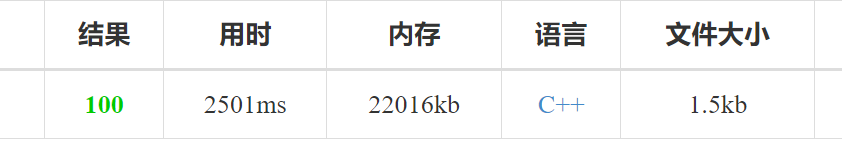
\includegraphics[width=0.8\textwidth]{fft1.png}
	\caption{fft-recursion \label{fig:fft1}}
\end{figure}

\lstinputlisting[language=C++, style=codestyle2]{code07/fft-recursion.cpp}


\subsubsection{FFT的迭代实现}
递归实现的 $FFT$ 效率不高,因为有栈的调用和参数的传递,实际中一般采用迭代实现。

{\heiti 二进制位翻转}

对分治规律的总结:
\begin{figure}[!htbp]
	\centering
	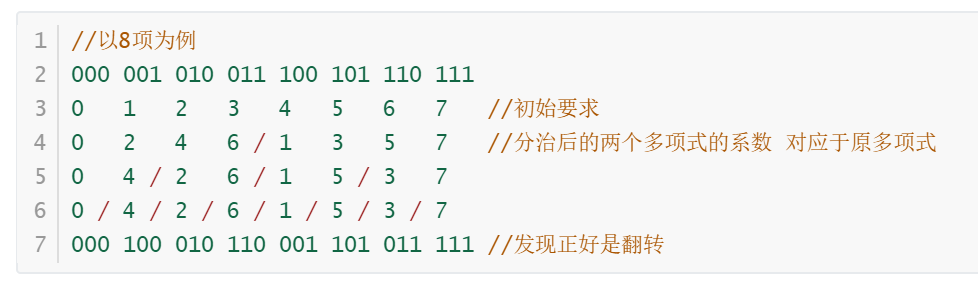
\includegraphics[width=1.0\textwidth]{fft-iter.png}
	\caption{分治的规律 \label{fig:fft-pattern}}
\end{figure}
这为迭代实现提供了理论基础。

{\heiti 蝴蝶操作}

考虑合并两个子问题的过程,假设$A_1(w_{\frac{n}{2}}^k)$ 和$A_2(w_{\frac{n}{2}}^k)$ 分别存放在$a[k]$和$a[\frac{n}{2}+k]$中,$A(w_n^k)$和$A(w_n^{k+\frac{n}{2}})$ 将要存放在$b[k]$和$b[\frac{n}{2}+k]$中,合并的操作可以表示为:
\begin{align*}
b[k]\leftarrow  a[k]+w_n^k*a[\frac{n}{2}+k]  \\
b[k+\frac{n}{2}] \leftarrow a[k]-w_n^k*a[\frac{n}{2}+k]
\end{align*}
考虑加入一个临时变量$t$,使得这个过程可以在原地完成,而不需要数组$b$,	
\begin{align*}
t \leftarrow w_n^k*a[\frac{n}{2}+k]   \\
a[k+\frac{n}{2}] \leftarrow a[k]-t  \\
a[k] \leftarrow a[k]+t
\end{align*}
由于$k$和$k+\frac{n}{2}$ 是对应的,所以不同的$k$之间不会相互影响。

这一过程被称为蝴蝶操作。

\begin{figure}[!htbp]
	\centering
	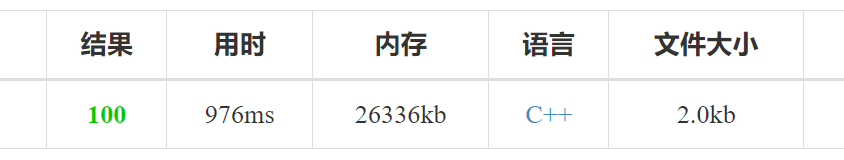
\includegraphics[width=0.8\textwidth]{fft2.png}
	\caption{fft-iteration \label{fig:fft2}}
\end{figure}

\lstinputlisting[language=C++, style=codestyle2]{code07/fft-iteration.cpp}

\subsection{NTT}
由于$FFT$涉及到复数运算,难免有精度问题,在计算一些高精度乘法的时候就有可能由于精度出现错误,这
便让我们考虑是否有在模意义下的方法,这就是{\heiti 快速数论变换}($Fast\ Number-Theoretic\ Transform,\ NTT$)。

首先来看$FFT$中能归并地变换用到了单位根$\omega_n$的什么性质:
\begin{enumerate}
\item $\omega_n^n = 1$;
\item $\omega_n^0\ ,\ \omega_n^1\ ,\ \omega_n^2\ ,\ ...\ ,\ \omega_n^{n-1}$是互不相同的,这样代入计算出来的点值才可以用来还原出多项式的系数;
\item $\omega_n^{k+\frac{n}{2}}=-\omega_n^{k}$,$\ \omega_{2n}^{2k}=\omega_n^k$,这使得问题规模得以减半;
\item $\sum_{i=0}^{n-1}(\omega_n^{j-k})^i = \left\{\begin{matrix}
0,\quad j\neq k\\ 
n,\quad j= k
\end{matrix}\right.$,这使得可以用同样的优化方法加速逆变换。
\end{enumerate}

下面我们要在模意义下寻找满足这些性质的数!

\subsubsection{原根}
由第三章中知一个素数$p$的原根$g$满足$g^0\ ,\ g^1\ ,\ ...\ ,\ g^{p-2}\ (mod\ p)$均不相同。对于一个素数$p$,将其
写成$p=k*2^m + 1$的形式,记$2^m=n$,有$g^{kn}\equiv 1\ (mod\ p)$。我们记$g_n = g^k$,则有$g_n^n\equiv 1\ (mod\ p)$。
由于$g$是$p$的原根,则$g_n^0\ ,\ g_n^1\ ,\ ...\ ,\ g_n^{n-1}$互不相同。

到这里我们发现,在模$p$意义下,$p$的原根$g$的$k$次方$g_n$,具有和单位根$\omega_n$一样的性质!上面已经说明了其具有性质1和性质2。下面说明性质3。

由于$g_n^n\equiv 1\ (mod\ p)$,所以$g_n^{\frac{n}{2}}\equiv 1\ or\ -1\ (mod\ p)$。又由于$g$是原根,则$g_n^{\frac{n}{2}}\equiv -1\ (mod\ p)$。
所以$g_n^{k+\frac{n}{2}}\equiv -g_n^{k}$得证。至于$g_{2n}^{2k}\equiv g_n^k$,只需证$g_n^2\equiv g_{\frac{n}{2}}$。这是比较显然的,因为$k=\frac{p-1}{2^m}$。

对于性质4,证明方法类似,大家可以自行尝试。

因此在$NTT$中,我们可以用原根$g$的$k$次方$g_n$代替$FFT$中的单位根$\omega_{n}$。

\subsubsection{NTT的实现细节}
在$FFT$中,需要预处理$N$项单位根的次幂及其共轭,对应地,$NTT$中也需要。即预处理$g_n^0\ ,\ g_n^1\ ,\ ...\ ,\ g_n^{n-1}$,以及对应的模$p$意义下的逆元。

$NTT$的代码相比$FFT$的代码变动很少。
\begin{note}
\begin{enumerate}
\item 最后逆变换完成后除$n$时,变为乘上$n$关于$p$的逆元即可;
\item $p=k*2^m + 1$中,最大能取到的$2^m$为能处理的结果多项式项数极限。如对于素数$998244353= 119 * 2^{23} + 1$, 最多能处理的$N = 2^{23}$。当$N<2^{23}$时,要将
多余的部分乘到$k$上;(常见的素数及其原根见附录表)
\item 由于实数域上的运算比复数域运算要快,所以$NTT$的运行时间理论上会比$FFT$少;(但由于有取模操作在,所以上述说明是玄学......)
\item 如果一个题目不用取模,使用$NTT$时要注意原本的答案是否会大于等于所选取的模数$p$。
\end{enumerate}
\end{note}

\begin{figure}[!htbp]
	\centering
	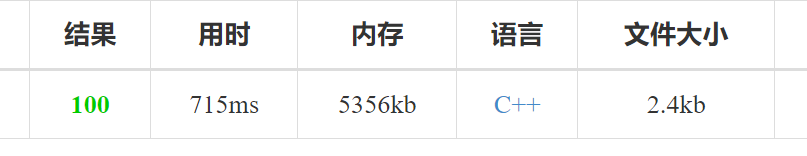
\includegraphics[width=0.8\textwidth]{ntt.png}
	\caption{NTT-iteration \label{fig:ntt}}
\end{figure}

\lstinputlisting[language=C++, style=codestyle2]{code07/NTT.cpp}

\subsubsection{模数任意的解决方案}
$NTT$要求模数写成$p=k*2^m + 1$的形式,但有些题目,要求模数写不成这样的形式,甚至是一个合数。
这样的话,一般选取$s$个常用的素数$p_1\ ,\ p_2\ ,\ ...\ ,\ p_s$,要求满足:
$$
\prod_{i=1}^s p_i > n(m-1)^2
$$
其中$n$是结果多项式的项数,$m$是要求的模数。然后分别在$mod\ p_i$下求解系数,最后使用中国剩余定理将结果合并(一般会使用高精度)。


%\section{多项式}

%\subsection{拉格朗日插值法}

%\subsection{多项式求逆}

%\subsection{多项式取模}

%\subsection{多项式开方}

%\subsection{多项式多点求值}

%\subsection{多项式多点插值}

\vbox{}

\vbox{}

\begin{problemset}
	\item \href{http://poj.org/problem?id=1305}{本原勾股数组 \quad poj 1305}
	\item 本原勾股数组 \quad fzu 1669
	\item \href{https://nanti.jisuanke.com/t/41421}{圆上整点/高斯素数 \quad 2019上海网络赛}
	\item \href{https://www.51nod.com/Challenge/Problem.html#problemId=1195}{斐波那契数列循环节 \quad 51nod-1195}
	\item dfs similar \quad 2019icpc亚洲区域赛-南昌站B题
	\item FFT \quad BZOJ 3992 / SDOI2015 序列统计
	\item FFT \quad BZOJ 3771 Triple
	\item \href{https://www.lydsy.com/JudgeOnline/problem.php?id=3527}{BZOJ 3527 \quad FFT}
	\item \href{https://www.luogu.com.cn/problem/P4245}{模板:任意模数NTT}
\end{problemset}


\nocite{*} 

\bibliography{reference}